\chapter{Security of the Diplomatiq application}
\label{chapter:security}

\section{Introduction}

\subsection{Motivation}

Web applications in general are notoriously insecure. According to an article by the prominent security firm Positive Technologies, statisticts of 2019 showed that hackers were able to hack users in 9 out of 10 web applications, exploiting vulnerabilities in the applications themselves~\cite{ptsecurity-2019}. The same article claims that breaches of sensitive data were a threat in 68\% of web applications, with the most breachable data being personal information and access credentials.

Having worked in cryptographic software development, I share the opinion that there is no such thing as too much software security. As on the one hand, Diplomatiq will store sensitive personal information from the beginning of its operation, and on the other hand, future diplomatic applications of the software will require strong security guarantees, I decided to put serious efforts to securing the Diplomatiq application. In this chapter, I present how I designed and implemented an application security framework addressing authentication, authorization, and data protection, providing cryptographic assurances regarding access control and the confidentiality and integrity of sensitive data.

\subsection{Scope and approach}

The implemented application security measures address all application layers across the front end and the back end of Diplomatiq. The front end needs to provide secure local data storage in the browser, as well as a variety of other security measures so the user can not be tricked into surrendering their password or other sensitive data. On the back end, the whole application needs to be secured, from the API's authentication and authorization mechanisms to the encrypted database records.

For securing the front end and the back end, I started off from my professional experience of securing a web application, and I also consulted the Open Web Application Security Project's web application security testing guide~\cite{owasp-webtestguide}. I implemented zero-knowledge user authentication using a suitable protocol, and I built a signing and authentication mechanism for HTTPS requests based on a symmetric cryptographic key hierarhcy, created upon the resulting shared key of the user authentication protocol. For authorizing sensitive API operations, I introduce the concept of session assurance level in order to make sure that the logged user is indeed themselves, and not an attacker who hijacked a user's session.

\section{Implemented cryptographic structures}

\subsection{DiplomatiqAEAD}

DiplomatiqAEAD is an \emph{Authenticated Encryption with Associated Data} structure, providing binary serialization and deserialiaztion capabilities. It essentially consists of an encrypted secret value and a public value attached to it, while the whole structure is authenticated, meaning it can not be modified without detection.

For the authenticated encryption, I chose today's prevalent Advanced Encryption Standard (AES) algorithm with 256-byte-long keys, in the more and more popular Galois/Counter Mode (GCM). AES-GCM provides strong confidentiality and ensures integrity of both the ciphertext and the additional authenticated data.

Although it does not contain self-implemented low-level cryptographic elements, DiplomatiqAEAD can be regarded as a cryptographic primitive within Diplomatiq applications, since it is a basic cryptographic building block of the system's authentication and database encryption infrastructure. The structure is used for transmitting encrypted and authenticated data across the front end and the back end application. This requires that the structure can be serialized in a self-contained way — meaning it must contain all necessary metadata needed for decryption as well —, and also that the two implementations on two different platforms are compatible with each other.

Similarly to other block cipher modes of operation, GCM also needs an initialization vector for a properly randomized output. According to the recommendation of the National Institute of Standards and Technology — a prevalent actor in cryptographic standards as well —, the initialization vector should be unique and 12 bytes long for efficient calculations~\cite{dworkin2007sp}. The initialization vector is also needed for decryption, so it needs to be included in the serialized packet. The output of AES-GCM is the ciphertext and an authentication tag, which is essentially a digest of the ciphertext, the initialization vector, and the additional authenticated data, verifying the integrity of all three. Most cryptography APIs append the authentication tag to the end of the ciphertext. As the authentication tag is needed for performing decryption, it needs to be included in the serialized packet.

For encoding the initialization vector, the ciphertext, the additional authenticated data and the authentication tag as a binary structure, I created a lightweight binary serialization scheme for DiplomatiqAEAD.\footnote{Although there are established standards like ASN.1, I decided that using it for this simple purpose only would cause more pain than gain.} The scheme consists of a header and a body. The body consists of the initialization vector, the additional authentication data, the ciphertext, and the authentication tag, in this order. Since each part of the body can essentially be of arbitrary length, the header contains each body part's length encoded on a fixed length: the length of the initialization vector on 1 byte, the length of the ciphertext on 4 bytes, the length of the additional authenticated data on 4 bytes, and the length of the authentication tag on 1 byte. All lengths are encoded in big-endian byte order, in unsigned magnitude representation. Encoding the length of the ciphertext and the additional authenticated data on 4 bytes introduces a planned constraint that DiplomatiqAEAD can be used only for encrypting and authenticating maximum 4 gigabytes of data at once. \Cref{fig:aead} presents the binary serialization format of DiplomatiqAEAD.

\begin{figure}[!htb]
    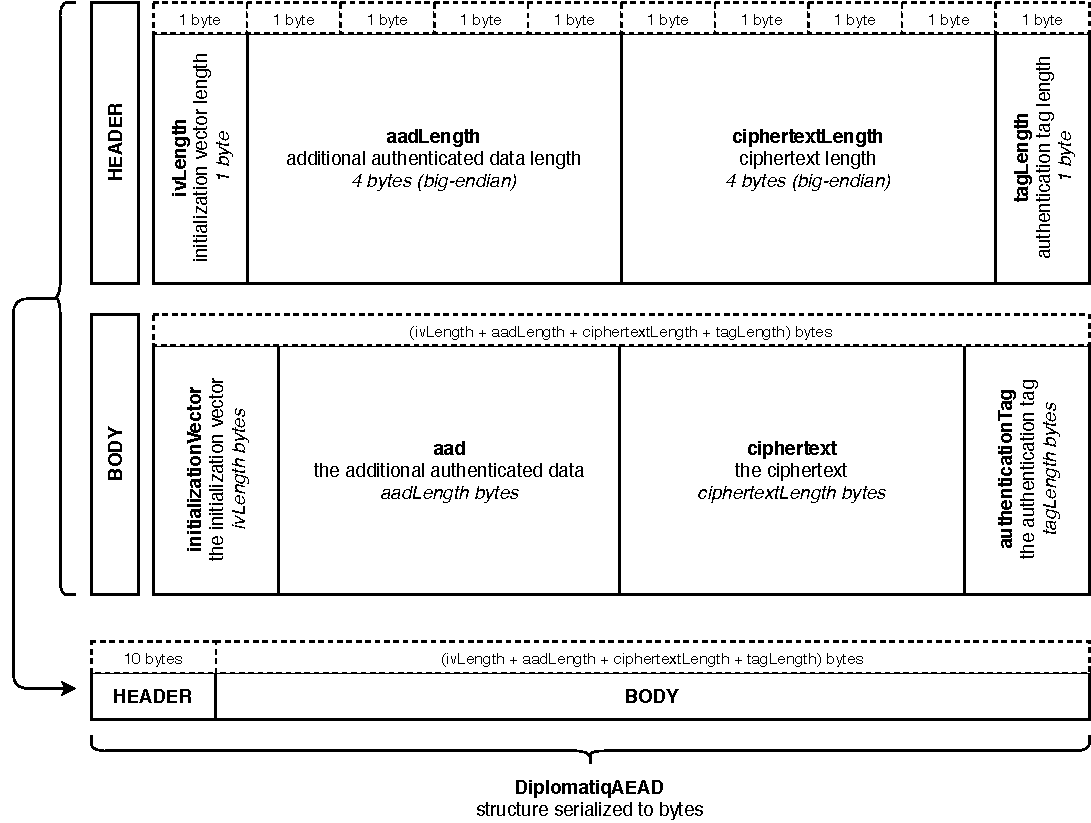
\includegraphics[width=\textwidth]{figures/aead.pdf}
    \caption{The structure of DiplomatiqAEAD serialized to bytes}
    \label{fig:aead}
\end{figure}

\section{Applied web platform security measures}

\subsection{Cross-Site Scripting (XSS)}

Cross-Site Scripting (XSS) attacks are a type of code injection, in which malicious scripts are injected into otherwise benign and trusted websites. XSS attacks occur when an attacker uses a web application to send malicious code, generally in the form of a browser side script, to an end user. Flaws that allow these attacks to succeed are quite widespread and occur anywhere a web application uses input from a user within the output it generates without validating or encoding it~\cite{owasp-xss}. Although in most modern browsers, a strong Content Security Policy ruleset disabling inline JavaScript can mitigate XSS, in older browsers the \lstinline{X-XSS-Protection} header can be used to instruct the browser to prevent rendering the page if an XSS attack is detected. Diplomatiq includes the \lstinline{X-XSS-Protection} header into its responses. The Angular framework also implements strong XSS mitigation measures: as long as their built-in filtering is used to display dynamic data in the browser, the application is protected. Diplomatiq uses Angular's built-in filtering.

\subsection{Content Security Policy (CSP)}

The Content Security Policy browser mechanism allows websites and web applications to specify what kind of resourcs (e.g. images, stylesheet files, script files, font files) can be loaded within the context of the application, and what kind of domains can the application connect to via network calls. This can protect against XSS attacks, and can also protect against performing unauthorized API calls. Diplomatiq applies a very strict Content Security Policy ruleset, which restricts everything by default, and only allows loading images, script files, stylesheet files, and font files from the application's very own domain name. Inline scripts are not allowed, meaning the application is safe against XSS attacks. Diplomatiq's policy allows connecting the front end application to \emph{api.diplomatiq.org} only.

\subsection{Cross-Origin Resource Sharing (CORS)}

By default, web browsers enforce the same-origin policy, meaning a web application running on a given domain can not initiate network requests to another domain. The Cross-Origin Resource Sharing mechanism instructs the browser to allow an application running on a certain origin to connect to a domain different than its origin. CORS settings are communicated to browsers via additional HTTP headers, specifying the origins which are allowed to connect to the domain which issued the headers. The Diplomatiq back end application issues CORS headers, which authorizes the application running under \emph{app.diplomatiq.org} to connect to the back end. No other application is authorized other than Diplomatiq's front end application.

\subsection{Feature Policy}

The Feature Policy experimental mecahnism enables to deny the usage of browser features for a web application, such as the browser's geolocation API, camera API, vibrate API, full screen API, etc. Feature Policy settings are communicated to the browser via a \lstinline{Feature-Policy} header. Their Feature Policies being the strictest, Diplomatiq's applications are not authorized to use such browser APIs at all.

\subsection{Referrer Policy}

The Referrer Policy mechanism can mitigate threats associated with the \lstinline{Referer}\footnote{The \lstinline{Referer} header is a misspelling of word \textquote{referrer}.} header. The \lstinline{Referer} header contains the URL of the page which the user visited before navigated to the current page. Referrer Policy settings are communicated to the browser via the \lstinline{Referrer-Policy} header. Their Referrer Policies being the strictest, Diplomatiq's applications omit the \lstinline{Referer} header entirely.

\subsection{Preventing click-jacking}

Click-jacking is a type of attacks where a page is embedded into another page via an \lstinline{<frame>} or \lstinline{<iframe>} element, and the user's clicks are hijacked to perform additional interactions on other web sites. Click-jacking can be prevented by instructing browsers not to allow embedding an application. Although Diplomatiq's restrictive Content Security Policy protects against this in modern browsers, in older browsers the \lstinline{X-Frame-Options} header should be set to \lstinline{DENY}. Diplomatiq's applications set this header accordingly as well.

\section{Authentication and authorization}

according to NIST https://nvlpubs.nist.gov/nistpubs/SpecialPublications/NIST.SP.800-63-3.pdf, multifactor authentication is necessary

oawsp top 10. listán 2. broken auth https://owasp.org/www-project-top-ten/

authentication why not oauth/openid/standard megoldások?

    1. signed requests and authentication

    2. session levels

    3. SRP

    4. cryptography

aláíráshoz az amazonos aláírásból indultam ki.

device container

\begin{figure}[!htb]
    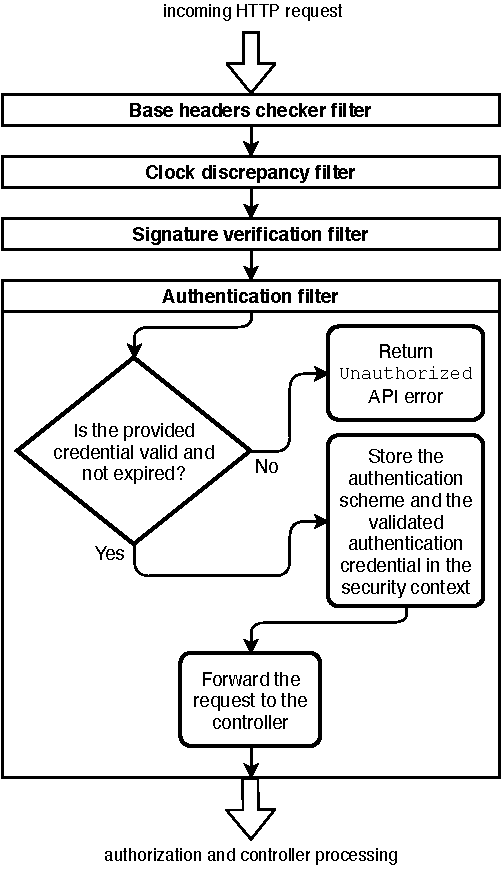
\includegraphics[width=\textwidth]{figures/authentication-filter.pdf}
    \caption{The authentication filter}
    \label{fig:authentication-filter}
\end{figure}

\begin{figure}[!htb]
    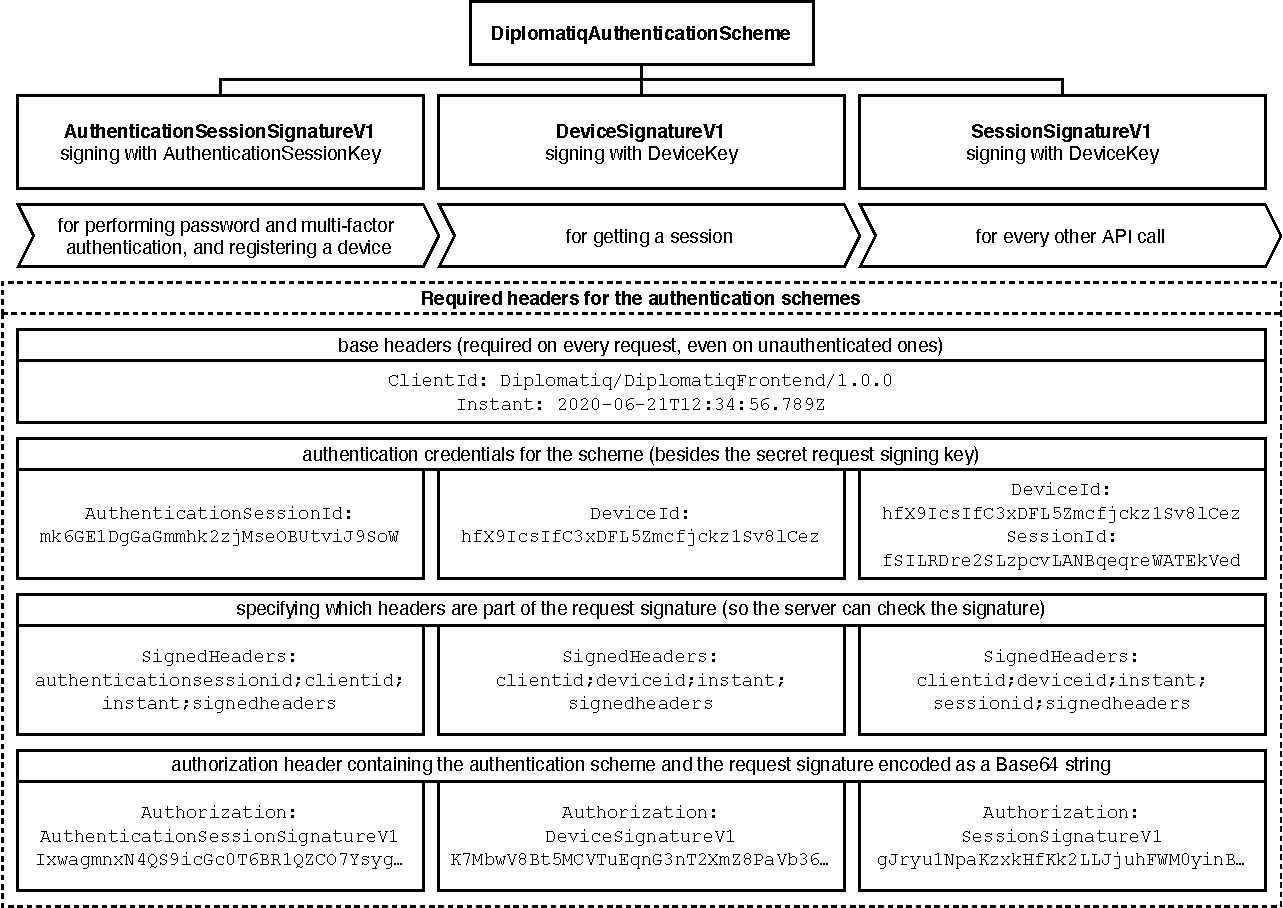
\includegraphics[width=\textwidth]{figures/authentication-schemes.pdf}
    \caption{A summary of Diplomatiq's authentication schemes}
    \label{fig:authentication-schemes}
\end{figure}

\begin{figure}[!htb]
    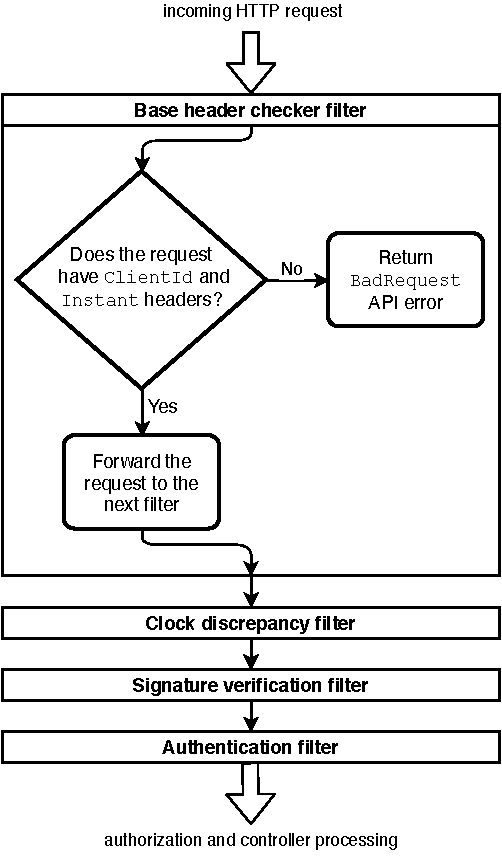
\includegraphics[width=\textwidth]{figures/base-headers-checker-filter.pdf}
    \caption{The base headers checker filter}
    \label{fig:base-headers-checker-filter}
\end{figure}

\begin{figure}[!htb]
    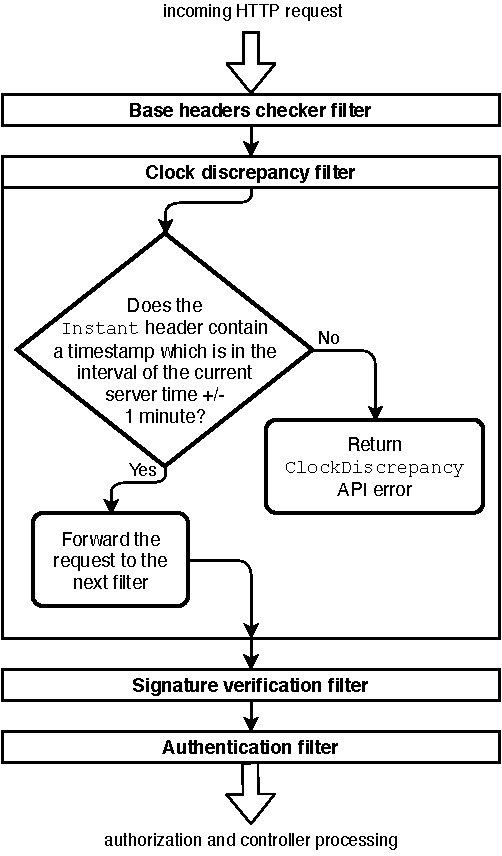
\includegraphics[width=\textwidth]{figures/clock-discrepancy-filter.pdf}
    \caption{The clock discrepancy filter}
    \label{fig:clock-discrepancy-filter}
\end{figure}

\begin{figure}[!htb]
    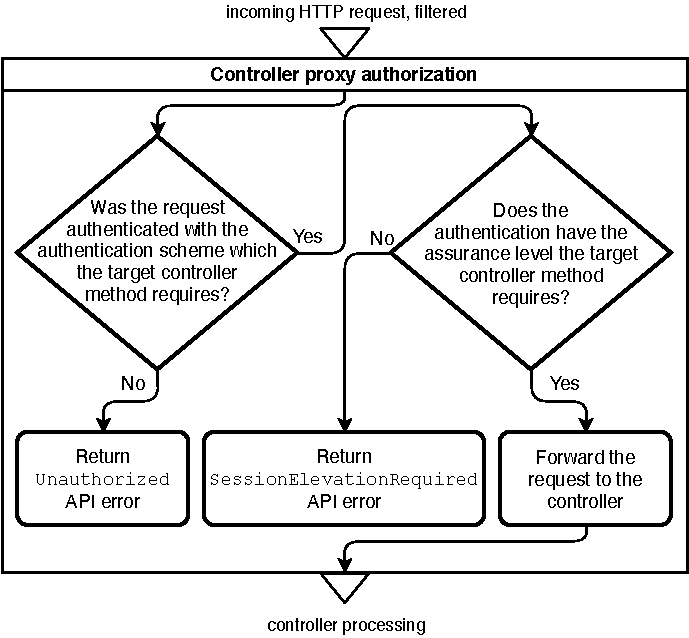
\includegraphics[width=\textwidth]{figures/controller-authorization.pdf}
    \caption{A summary of controller authorization}
    \label{fig:controller-authorization}
\end{figure}

\begin{figure}[!htb]
    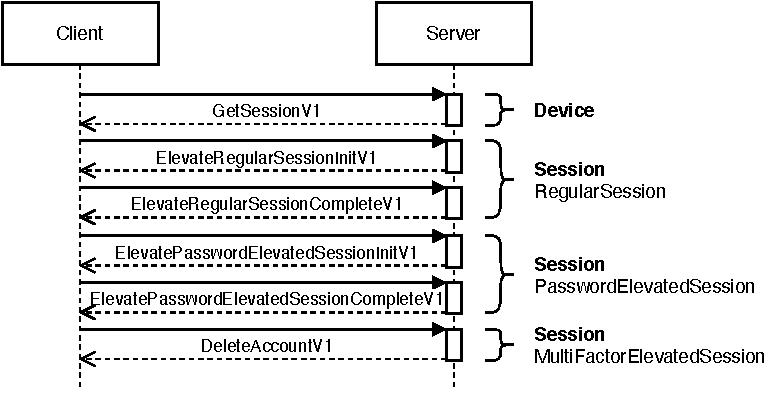
\includegraphics[width=\textwidth]{figures/elevate-to-mfa-session.pdf}
    \caption{Server calls for elevating a session to multi-factor level}
    \label{fig:elevate-to-mfa-session}
\end{figure}

\begin{figure}[!htb]
    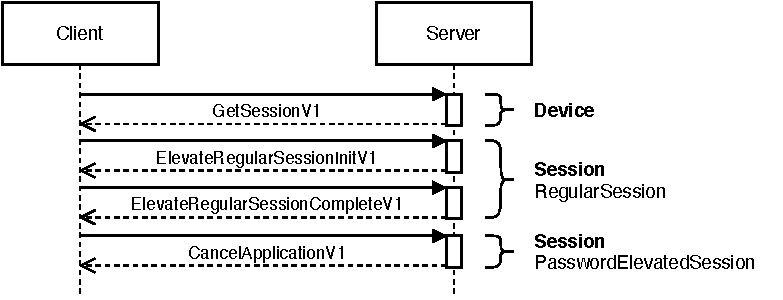
\includegraphics[width=\textwidth]{figures/elevate-to-password-session.pdf}
    \caption{Server calls for elevating a session to password level}
    \label{fig:elevate-to-password-session}
\end{figure}

\begin{figure}[!htb]
    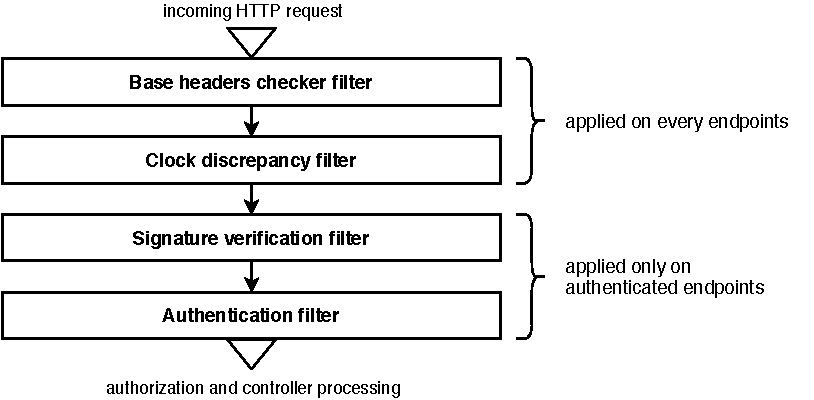
\includegraphics[width=\textwidth]{figures/request-filters.pdf}
    \caption{A summary of the back end application's request filters}
    \label{fig:request-filters}
\end{figure}

\begin{figure}[!htb]
    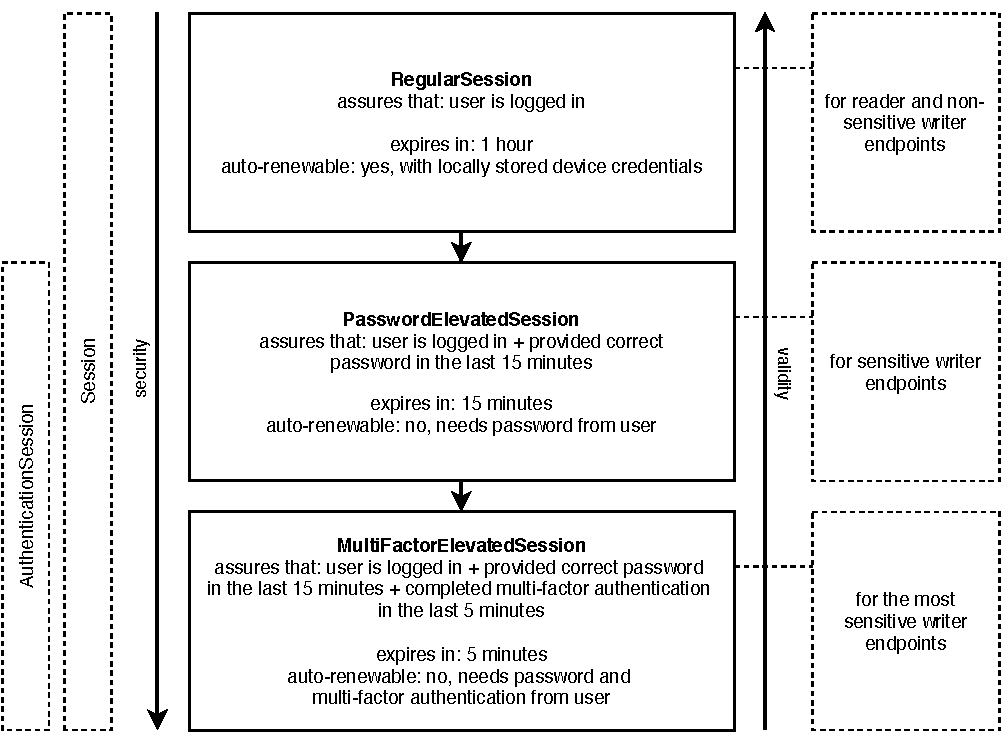
\includegraphics[width=\textwidth]{figures/session-assurance-levels.pdf}
    \caption{Diplomatiq's session assurance levels}
    \label{fig:session-assurance-levels}
\end{figure}

\begin{figure}[!htb]
    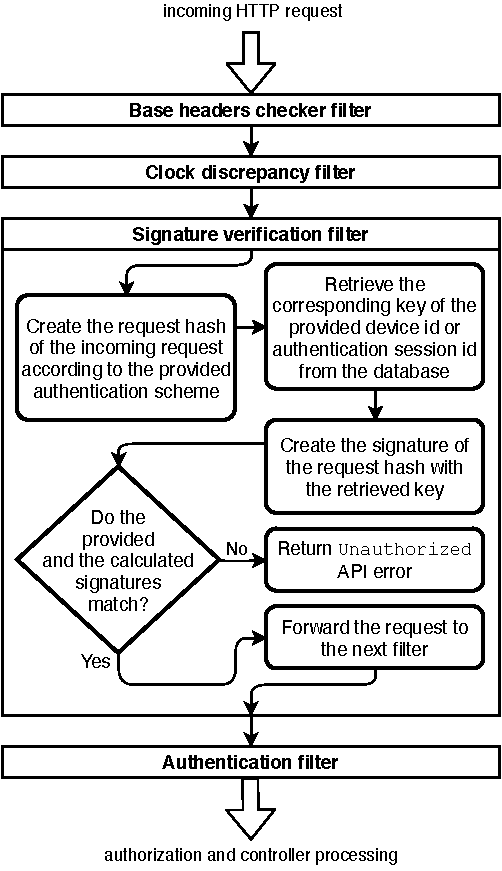
\includegraphics[width=\textwidth]{figures/signature-verification-filter.pdf}
    \caption{The signature verification filter}
    \label{fig:signature-verification-filter}
\end{figure}

\section{Encrypting sensitive data in the database}

encrypted db values, key versioning to avoid birthday problem

\section{Other security measures}

nem adunk ki a userről adatot (hogy létezik-e ilyen mailcímű user, stb)

security.txt
